\documentclass[12pt]{article}
\usepackage{import}
\usepackage{preamble}
\usepackage{environments}
%\usepackage{fourier}

%hspace before small will move the keywords around
\providecommand{\keywords}[1]
{
    \hspace*{0pt}\small	
  \textbf{\textit{Keywords--}} #1
}

\title{Differential forms and Stokes' Theorem in $\R^3$}
\renewcommand{\maketitlehookb}{\centering Greenslopes Graduate Student Seminar\\
Colorado State University}
\author{Colin Roberts}
\date{September 5$^\textrm{th}$ 2019}


\begin{document}

% Title Page
\begin{titlingpage}
    \maketitle
    \vfill
    \begin{abstract}
       When learning multivariate calculus, we work with vectors and products of vectors to represent physical quantities.  Of course, calculus then drives to see how these quantities can change from point to point.  The main issue is that $\R^3$ is especially nice and, due to this, it does not generalize without quite a bit more work. The goal is then to build a proper, and generalizable, notion of differential and integral calculus in $\R^3$.  Our key tool will be differential forms.  Think of forms as coordinate free measuring sticks that can be placed in not only $\R^3$ but also any $n$-dimensional manifold.  Forms have a rich algebraic structure and they can be differentiated and integrated. After defining forms somewhat heuristically, we will investigate the wedge product and exterior derivative. The exterior derivative will give us a cochain map on the de Rham cochain complex and we briefly mention the de Rham cohomology. Then, we can realize the different forms of the Fundamental Theorem of Calculus (divergence and Stokes' theorem) under the guise of a more modern Stokes' theorem formulated by \'Ellie Cartan.
    \end{abstract}
    %\vspace*{10pt}
    \keywords{vectors, dual vectors, differential $k$-form, wedge product, exterior derivative, de Rham cohomology, Stokes' theorem}
\end{titlingpage}

% \section*{Outline}
% \begin{enumerate}[1.]
%     \item Introduce smooth manifolds by building up from topological spaces.
%     \item Define bundles generally and then introduce the canonical bundles $TM$ and $T^*M$.
%     \item Realize the space of sections of $TM$ and $T*M$ form a $C^\infty(M)$-module.
%     \item Build the tensor product of bundles and tensor product of the spaces of sections.
%     \item Show the examples of the (0,2)-tensor bundle and the $k$-exterior power bundle and their sections.
%     \item Mention the tensor algebra and quotients and consider the construction on $M$.
% \end{enumerate}

\section{Introduction}

\subsection{Motivation}
Different measuring sticks should not change the physics.  This is roughly what one means when stating that we work in a coordinate free way.  Our measuring sticks, in this context, will be \emph{differential forms} (often just \emph{forms}). If you have ever wondered what $dx$ represents, then the material here will start to lead you there. 

Though the language of forms is rather unnecessary in $\R^3$, it gives us the opportunity to understand the meaning behind them so that we can utilize them in settings where there is no better option.  When working on manifolds, they are of utmost importance when considering integration or differential equations.  

Where appropriate, I will be general.  Otherwise, I will stick to the specific case of $\R^3$ and possible $\R^2$.

There are apparent problems with the vector algebra and calculus that we hardly ever mention.  
\begin{ques}{}{ques1}
    How do you really define the curl of two vectors in $\R^3$?
    \tcblower
    \begin{answer*}
    Naively, we can take $\times \colon \R^3 \times \R^3 \to \R^3$ and define the map as per usual.  That is, given $\mathbf{v}=(v_1,v_2,v_3)$ and $\mathbf{w}=(w_1,w_2,w_3)$,
    \[
    \mathbf{v}\times \mathbf{w} = (v_2w_3-v_3w_2,v_3w_1-v_1w_3,v_1w_2-v_2w_1).
    \]
    But, this can't be quite right.  Say if we consider angular momentum 
    \[
    \mathbf{L}=\mathbf{r}\times \mathbf{p},
    \]
    then $\mathbf{r}$ and $\mathbf{p}$ don't even belong to the same space since they have completely different units! And the output $\mathbf{L}$ doesn't share the same dimensions as either $\mathbf{r}$ or $\mathbf{p}$. What's the deal?
    
    So we could play off the fact by saying we really have $\times \colon V \times W \to Z$ where $V\cong W \cong Z \cong \R^3$ as vector spaces but we understand that the underlying spaces have dimensions of their own and that the binary operation of $\times$ outputs to a new space with the correct dimensions. 
    \end{answer*}
\end{ques}



It turns out that differential forms and the \emph{exterior} algebra capture this all quite nicely without having to make note  of this extra structure so explicitly.  Also, vector curl does not even exist in any dimension other than three, thus if we wish to talk about vorticity in higher dimensions, we need something else.

Vector calculus is also captured nicely in the same way. One can repeat the same above question but instead consider the curl $\curl$ of a vector field.  The answer will be analogous in that the \emph{exterior derivative} plays the role of the curl.  In fact, it will take over the role of the gradient $\nabla$, curl, and divergence $\diver$.

\subsection{Preliminaries}

One should feel comfortable with the notions presented in a first multivariate calculus course. Namely, the following:
\begin{itemize}
    \item \emph{Smooth multivariate functions}, $f\colon \R^n \to \R^m$. Here, we mostly concern ourselves with \emph{scalar functions} $f\colon \R^3\to \R$ or \emph{vector fields} $\vfield \R^3 \to \R^3$. Of course, functions may be defined only on (nice) subsets $\region \subset \R^n$.  
    \item \emph{Gradient}, \emph{curl}, and \emph{divergence}.  That is, given a scalar field $f$, we can compute the gradient
    \[
    \nabla f = \left(\frac{\partial f}{\partial x}, \frac{\partial f}{\partial y}, \frac{\partial f}{\partial z}\right).
    \]
    Given a vector field $\vfield$, we can compute the curl
    \[
    \curl \vfield = \left(\frac{\partial F_3}{\partial y}-\frac{\partial F_2}{\partial z}, \frac{\partial F_1}{\partial z}-\frac{\partial F_3}{\partial x}, \frac{\partial F_2}{\partial x}-\frac{\partial F_1}{\partial y}\right),
    \]
    or
    \[
    \diver \vfield = \frac{\partial F_1}{\partial x}+\frac{\partial F_2}{\partial y}+\frac{\partial F_3}{\partial z}.
    \]
    Exactly what these mean is not totally necessary, but familiarity would be ideal.
    \item \emph{Vector spaces} and their corresponding \emph{dual vector spaces}. We only care about $\R^n$ here and its dual $\left(\R^n\right)^*$.  The dual space is defined as
    \[
    \left(\R^m\right)^* \coloneqq \{ \varphi \colon \R^m \linmap \R\},
    \]
    where we let $\linmap$ represent a \emph{linear map}. We typically call elements $\omega \in \left(\R^n\right)^*$ \emph{dual vectors} or \emph{covectors}.
\end{itemize}

\section{Differential Forms}

\subsection{Set Up}
Consider a region in $n$-space, $\region \subseteq \R^n$. Let $p\in \region$, then we can define the \boldblue{tangent space at $p$}, $\tangentspace$, to be the set of all vectors that are based at the point $p$. That is, vectors whose tails are attached at the point $p$ and are free to point in any direction and have any magnitude. Since $\region \subseteq \R^n$, the tangent space can be identified with $\R^n$ itself and we write $\tangentspace \cong \R^n$. Then, we call elements $\tangentvect \in \tangentspace$ \boldblue{tangent vectors at $p$}. Different points correspond to different tangent spaces, and thus we could also have a tangent vector $\mathbf{Y}_q\in T_q\region$.

        \begin{figure}[ht]
        \centering
        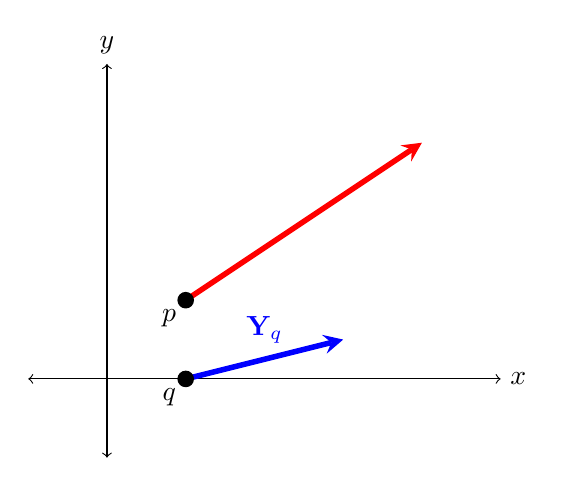
\begin{tikzpicture}
        \centering
        \draw node[anchor=north east] at (1,1){$p$};
        \draw[<->] (-1,0)--(5,0) node[right]{$x$};
        \draw[<->] (0,-1)--(0,4) node[above]{$y$};
        \draw[line width=2pt,red,-stealth](1,1)--(4,3) node[anchor=south east] at (2.5,2.1){$\tangentvect$};
        \fill (1,1) circle[radius=3pt];
        \draw node[anchor=north east] at (1,0){$q$};
        \draw[line width=2pt,blue,-stealth](1,0)--(3,.5) node[anchor=south] at (2,.3){$\mathbf{Y}_q$};
        \fill (1,0) circle[radius=3pt];
        \end{tikzpicture}
        \caption{Figure 1: Tangent vectors in different tangent spaces.}
        \end{figure}
        
\begin{remark}{}{rem1}
One of the fundamental issues in differential geometry is comparing vectors in different tangent spaces.  One needs a \emph{connection} to do this properly.  In $\R^n$, this connection is trivial.  There, we can simply drag any vector to the origin without extra thinking.
\end{remark}

Now, we can dualize this setting as well.  We define the \boldblue{cotangent space at $p$}, $\cotangentspace$, to be the set of all covectors based at the point $p$.  More concretely, these covectors are real valued functions that eat tangent vectors and output real numbers. Hence,
\[
\cotangentspace \coloneqq \{\covect \colon \tangentspace \linmap \R\}.
\]

For $\tangentspace$, we can choose an arbitrary basis $e_{1_p},\dots, e_{n_p}$. Often, we will just assume that this basis is the standard orthonormal basis at that point.


\begin{figure}[ht]
\centering
        \begin{tikzpicture}
        \fill (1,1) circle[radius=3pt];
        \draw node[anchor=north east] at (1,1){$p$};
        \draw[<->] (-1,0)--(5,0) node[right]{$x$};
        \draw[<->] (0,-1)--(0,4) node[above]{$y$};
        \draw[line width=2pt,red,-stealth](1,1)--(4,3) node[anchor=south east] at (2.5,2.1){$\tangentvect$};
        \draw[line width=2pt, black, -stealth](1,1)--(2,1) node[anchor=west] at (2,1){$e_{1_p}$};
        \draw[line width=2pt, black, -stealth](1,1)--(1,2) node[anchor=south] at (1,2){$e_{2_p}$};
        \end{tikzpicture} 
    \caption{Figure 2: A tangent vector $\tangentvect$ and the standard basis vectors at the point $p$. These are all vectors in $\tangentspace$.}
\end{figure}


\noindent Then, we can construct the \emph{dual basis} of covectors $dx^1,\dots,dx^n_p$ by forcing
\[
dx^i_p\left(e_{j_p}\right)=\delta^i_j = 
\begin{cases}
0, & i\neq j\\
1, & i=j
\end{cases}.
\]
This is a standard construction of a dual basis.

We can define a \boldblue{vector field}, $\vectfield$, by smoothly choosing a tangent vector $\tangentvect$ at each point $p\in \region$.  Thus we can put
\[
\tangentvect = \tangentvect= \sum_{i=1}^n f_i(p)e_{i_p}.
\]
Since we are working over a region in $\R^n$, we can let $e_{i_p}$ be the $i$th standard basis vector at each point and then $f_i$ is simply a smooth scalar function (i.e., $f_i\in \cinfinity$). Then we denote by $\vectfields$ the set of all vector fields on the region $\region$. 

        \begin{figure}[ht]
        \centering
        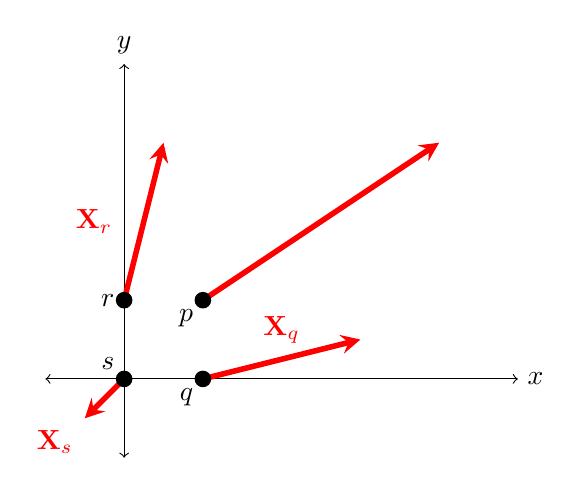
\begin{tikzpicture}
        \draw node[anchor=north east] at (1,1){$p$};
        \draw[<->] (-1,0)--(5,0) node[right]{$x$};
        \draw[<->] (0,-1)--(0,4) node[above]{$y$};
        \draw[line width=2pt,red,-stealth](1,1)--(4,3) node[anchor=south east] at (2.5,2.1){$\tangentvect$};
        \fill (1,1) circle[radius=3pt];
        \draw node[anchor=north east] at (1,0){$q$};
        \draw[line width=2pt,red,-stealth](1,0)--(3,.5) node[anchor=south] at (2,.3){$\mathbf{X}_q$};
        \fill (1,0) circle[radius=3pt];
        \draw node[anchor=east] at (0,1){$r$};
        \draw[line width=2pt,red,-stealth](0,1)--(.5,3) node[anchor=east] at (0,2){$\mathbf{X}_r$};
        \fill (0,1) circle[radius=3pt];
        \draw node[anchor=south east] at (0,0){$s$};
        \draw[line width=2pt,red,-stealth](0,0)--(-.5,-.5) node[anchor=north east] at (-.5,.-.5){$\mathbf{X}_s$};
        \fill (0,0) circle[radius=3pt];
        \end{tikzpicture}
        \caption{Figure 3. A few tangent vectors from a vector field $\mathbf{X}$.}
        \end{figure}

\subsection{Differential 1-Forms}

A \boldblue{differential 1-form} (henceforth, 1-form) is a cotangent vector field. Analogous to a vector field, a 1-form is defines a covector at each point in $\region$. We say that a 1-form is \emph{smooth} if it varies smoothly from point to point in the same way a vector field does. Analogously, we put
\[
\covect \coloneqq \sum_{i=1}^n g_i(p)dx^i_p,
\]
where $g_i\in \cinfinity$ is smooth. We will let $\oneforms$ denote the space of 1-forms on the region $\region$.

\begin{ex}{Basis 1-Forms in $\R^2$}{basis_forms_R^2}
Consider $\region = \R^2$ with $e_{1_p}$ and $e_{2_p}$ the standard basis for $\tangentspace$. Then let $dx_p$ and $dy_p$ denote the dual basis in $\cotangentspace$. Let us say that we have the tangent vector $\tangentvect$ which can be identified as the vector
\[
\tangentvect = 3e_{1_p}+2e_{2_p}.
\]
Then the basis 1-forms produce the following:
\begin{align*}
    dx_p(\tangentvect)&=dx_p(3e_{1_p}+2e_{2_p})=3dx_p(e_{1_p})+2\underbrace{dx_p(e_{2_p})}_{=0}=3\\
    dy_p(\tangentvect)&=dy_p(3e_{1_p}+2e_{2_p})=3\underbrace{dy_p(e_{1_p})}_{=0}+2dy_p(e_{2_p})=2.\\
\end{align*}
        \begin{center}
        \begin{tikzpicture}
        \draw node[anchor=north east] at (1,1){$p$};
        \draw[<->] (-1,0)--(5,0) node[right]{$x$};
        \draw[<->] (0,-1)--(0,4) node[above]{$y$};
        \draw[line width=2pt,red,-stealth](1,1)--(4,3) node[anchor=south east] at (2.5,2.1){$\tangentvect$};
        \draw[dashed] (4,1)--(4,3) node[anchor=west] at (4,2){$dy_p(\tangentvect)=2$};
        \draw[dashed] (1,1)--(4,1) node[anchor=north] at (2.5,1){$dx_p(\tangentvect)=3$};
        \fill (1,1) circle[radius=3pt];
        \end{tikzpicture}
        \end{center}
        Of course, we can then define a 1-form 
        \begin{align*}
        \covectfield(p)&=g_1(p)dx_p+g_2(p)dy_p.
        \end{align*}
        Then letting $p=(p_1,p_2)$ we could define, for example,
        \begin{align*}
            g_1(p)&=(p_1+1)^2\\
            g_2(p)&=5p_2.
        \end{align*}
        Letting $p=(1,1)$ specifically, we have
        \[
        \boldsymbol{\omega}_{p}=4dx_p+5dy_p.
        \]
        Then
        \begin{align*}
        \covect(\tangentvect)&=4\cdot 3dx_p\left(e_{1_p}\right)+5\cdot 2dy_p\left(e_{2_p}\right)\\
        &=22.
        \end{align*}
        \end{ex}
        
        \begin{remark}{}{rem2}
        1-forms have given us a way of measuring lengths of tangent vectors.  Also, they allows us to apply functions to the different components of vectors.  However, we want to be able to investigate areas and volumes as well. 
        \end{remark}
        
        \begin{ex}{1-Forms as Measurements}{one_form_measurements}
        Consider the 1-forms 
        \[
        \omega = xdx + y dy \qquad \textrm{and} \qquad \eta = -ydx + xdy
        \]
        which can serve as measurements for the divergence or curl (resp.) of a vector field $X$ about the origin.  
        \end{ex}
        
        We can also realize a 1-form by the \emph{differential} of a function.  If we consider a function
        \[
        f\colon \region \to \R
        \]
        then the \boldblue{differential at $p$} $df_p$ is a map
        \[
        df_p \colon \tangentspace \to T_{f(p)}\R
        \]
        where $T_{f(p)}\R$ is the tangent space of $\R$ at the point $f(p)$. However, we have that $T_{f(p)}\R\cong \R$ and so we can realize 
        \[
        df_{p} \colon \tangentspace \to \R,
        \]
        which means that $df_p$ is a cotangent vector at $p$.  In fact, going through the work shows that for $\region \subset \R^n$, and $f\colon \region \to \R$ we have
        \[
        df_p = \frac{\partial f(p)}{\partial x^1}dx^1 + \cdots + \frac{\partial f(p)}{\partial x^n}dx^n.
        \]
        If $f \in \cinfinity$ then $df$ is a smooth 1-form defined for each $p$.

\subsection{Wedge Product}

In order to measure areas and volumes, we need forms of higher degree. Given two 1-forms $\covectfield$ and $\covectfieldnew$ we can combine them in order to make a \boldblue{2-form}.  A 2-form will measure area, but in order to do so properly we need to construct this product of 1-forms correctly.  We define the \boldblue{wedge product} $\wedge$ of two 1-forms by writing a formal symbol
\[
\covectfield \wedge \covectfieldnew,
\]
and forcing the anti-symmetry relationship
\[
\covectfield \wedge \covectfieldnew = - \covectfieldnew \wedge \covectfield.
\]
Note that this also implies that
\[
\covectfield \wedge \covectfield = 0.
\]

\begin{remark}{}{rem3}
The wedge product is really a product in quotient of the tensor product of two vector spaces.  We have
\[
V \wedge V \coloneqq \bigslant{V\otimes V}{\langle v\otimes v \rangle}.
\]
We can let $V=\cotangentspace$ and glue these new vector spaces together to achieve what we have above with forms.
\end{remark}

\begin{ex}{Wedge Product in $\R^2$}{wedge_r^2}
For now, let us assume that $dx$ and $dy$ are global basis $1-forms$ in $\R^2$. Then, let
\[
\covectfield = Adx+Bdy \quad \textrm{and} \covectfieldnew = Cdx+Ddy,
\]
and take the wedge
\begin{align*}
    \covectfield \wedge \covectfieldnew &= (Adx+Bdy)\wedge (Cdx+Ddy)\\
    &=\underbrace{ACdx\wedge dx}_{=0} +ADdx\wedge dy +BC dy\wedge dx + \underbrace{BD dy\wedge dy}_{=0}\\
    &= (AD-BC)dx\wedge dy.
\end{align*}
Note that, up to a sign, $dx\wedge dy$ is the \emph{only} 2-form in $\R^2$.\\

Letting the base point be $p$ points and thinking of $dx$ as $e_{1_p}$ and $dy$ as $e_{2_p}$, we have the following geometric interpretation.
\begin{center}
        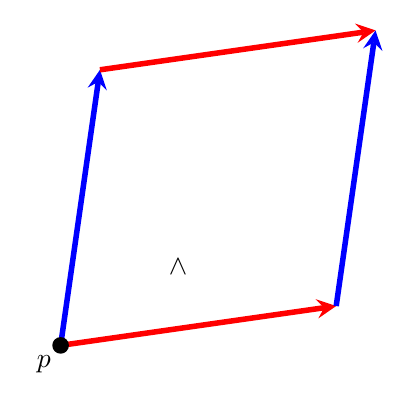
\begin{tikzpicture}
        \centering
        % \draw[<->] (-1,0)--(5,0) node[right]{$x$};
        % \draw[<->] (0,-1)--(0,4) node[above]{$y$};
        \draw[line width=2pt,red,-stealth](0,0)--(3.5,.5) node[anchor=north] at (2,.1){$\covectfield$};
        \draw[line width=2pt,blue,-stealth](0,0)--(.5,3.5) node[anchor=east] at (.1,2){$\covectfieldnew$};
        \draw[line width=2pt,red,-stealth](.5,3.5)--(4,4) node[anchor=south east] at (2.5,2.1){};
        \draw[line width=2pt,blue,-stealth](3.5,.5)--(4,4) node[anchor=south] at (2,.3){};
        \fill (0,0) circle[radius=3pt];
        \tdplotdrawarc[->,line width = 1pt]{(2,2)}{0.5}{45}{375}{}{};
        \node[anchor=west] at (1.25,1){$\covectfield \wedge \covectfieldnew$};
        \node[anchor=north east] at (0,0){$p$};
        \end{tikzpicture}
\end{center}
We can think of the two form $\covectfield \wedge \covectfieldnew$ as an oriented plane element that has area $|AD-BC|$.
\end{ex}

\begin{ques}{}{ques2}
\begin{itemize}
    \item Do we recognize $AD-BC$?
    \item If $dx$ and $dy$ both have units meters, then what should the units of $dx\wedge dy$ be?
\end{itemize}
\tcblower
\begin{answer*}~
\begin{itemize}
    \item AD-BC is exactly the determinant of a $2\times 2$ matrix. Recall that if we build the matrix with vectors as columns, then the determinant gives the area of the parallelogram constructed from those vectors.
    \item $dx\wedge dy$ should have units of square meters since it is a product.  We also desired this 2-form to measure area, so it should output the correct units.
\end{itemize}
\end{answer*}
\end{ques}



\subsection{k-Forms}

Given the ability to combine 1-forms, we can now combine forms of higher degree as well.  There are also 0-forms which we can consider as well.  However, a zero form contains no covector part, and is just a scalar function. So we let $\zeroforms$ denote the space of 0-forms but recognize that we identify
\[
\zeroforms \cong \cinfinity.
\]

We will say that a \boldblue{$k$-form} is a linear combination of wedge products of $k$ 1-forms.  That is, if $\covectfield$ is a $k$-form, then
\[
\covectfield = \sum_{I\in \mathcal{I}} f_I dx^{I},
\]
where $\mathcal{I}$ is collection of sets $I=\{i_1,\dots,i_k\}$, $f_I$ is a smooth scalar function for each $I$, and $dx^I$ is a wedge product of $k$-differential forms $dx^{i_1}\wedge \dots \wedge dx^{i_k}$. Then the space of $k$-forms on the region $\region$ is denoted by $\kforms$.  The role of a $k$-form is to measure an infinitesimal \emph{$k$-dimensional volume}.  Hence why we saw a 2-form measured area and would also have that a 3-form measures volume.

All $k$-forms can be integrated.  This is by design! Specifically, a $k$-form can be integrated over a $k$-dimensional manifold $M$.  For example, in $\R^3$, we could integrate a 3-form $\covectfield = hdx\wedge dy \wedge dz$ over a volume $V$
\[
\int_V \covectfield = \int_V hdx\wedge dy \wedge dz = \int_V h(x,y,z)dxdydz.
\]
Or, we could measure a 1-form $\covectfieldnew=f(x,y,z)dx$ over an interval $I$ by
\[
\int_I \covectfieldnew = \int_I f(x,y,z)dx.
\]
This is how we can measure volumes in varying dimensions. Of course, there are some subtleties in choosing a measure underlying all of this.

\begin{remark}
The spaces of $k$-forms $\kforms$ are all vector spaces.  In general, their dimension is given by
\[
\dim \left( \kforms\right) = \binom{n}{k}
\]
\end{remark}

\begin{ex}{$k$-Forms in $\R^3$}{kforms_r^3}
The basic $k$-forms we can have in $\R^3$ are the following:
\begin{itemize}
    \item 0-forms: $1$;
    \item 1-forms: $dx$, $dy$, and $dz$;
    \item 2-forms: $dx\wedge dy$, $dx\wedge dz$, and $dy\wedge dz$;
    \item 3-forms: $dx\wedge dy \wedge dz$.
\end{itemize}
\end{ex}

\subsection{Exterior Derivative}

These are \emph{differential} forms, so, from the name alone, we should expect some notion of a derivative.  The \boldblue{exterior derivative} is a map
\[
d\colon \kforms \to \Omega^{k+1}(\region)
\]
that satisfies
\begin{enumerate}[(i)]
    \item $df$ is the differential of $f$ for 0-forms.
    \item $d\circ d=0$.
    \item $d(\covectfield \wedge \covectfieldnew)=d\covectfield \wedge \covectfieldnew + (-1)^k(\covectfield \wedge d\covectfieldnew)$, where $\covectfield$ is a $k$-form.
\end{enumerate}
Rather than define the exterior derivative in full generality, it is nice to see it defined on forms in $\R^3$.  From here, it can be generalized without too much work.  

\begin{ex}{Exterior Derivative in $\R^3$}{ext_der_r^3}
Let us work through the exterior derivative on forms in increasing degree. For this, let $\region \subseteq \R^3$. In a way, you can think of $d$ as
\[
d = \frac{\partial \bullet}{\partial x} dx\wedge + \frac{\partial \bullet}{\partial y} dy\wedge + \frac{\partial \bullet}{\partial z} dz\wedge,
\]
where $\bullet$ represents an input for a scalar function. This is similar to a Dirac operator.
\begin{itemize}
    \item 0-forms. Let $f\in \cinfinity$, then
    \[
    df \coloneqq \frac{\partial f}{\partial x}dx + \frac{\partial f}{\partial y} dy + \frac{\partial f}{\partial z} dz.
    \]
    It turns out that $df$ is analogous to the gradient $\nabla$.
    \item 1-forms. Let $\covectfield = f_1dx+f_2dy+f_3dz$ be a 1-form. Then,
    \begin{align*}
        d\covectfield &\coloneqq \left( \frac{\partial f_1}{\partial x}dx\wedge dx + \frac{\partial f_1}{\partial y}dy\wedge dx+\frac{\partial f_1}{\partial z}dz\wedge dx \right)\\
        &\quad +\left( \frac{\partial f_2}{\partial x}dx\wedge dy + \frac{\partial f_2}{\partial y}dy\wedge dy+\frac{\partial f_2}{\partial z}dz\wedge dy \right)\\
        &\quad + \left( \frac{\partial f_3}{\partial x}dx\wedge dz + \frac{\partial f_3}{\partial y}dy\wedge dz+\frac{\partial f_3}{\partial z}dz\wedge dz \right)\\
        &=\left( \frac{\partial f_3}{\partial y}-\frac{\partial f_2}{\partial z}\right)dy\wedge dz + \left(\frac{\partial f_1}{\partial z}-\frac{\partial f_3}{\partial x}\right) dz\wedge dx + \left( \frac{\partial f_2}{\partial x} -\frac{\partial f_1}{\partial y}\right) dx\wedge dy.
    \end{align*}
    Note that if we identify $e_1 \equiv dy\wedge dz$, $e_2\equiv dz\wedge dx$, and $e_3\equiv dx\wedge dy$, then this is the curl $\nabla \times$.
    \item 2-forms. With the same identification of $e_1$, $e_2$, and $e_3$ above, we let $\covectfield = g_1 dy\wedge dz + g_2 dz\wedge dx + g_3 dx\wedge dy$. Then,
    \begin{align*}
        d\covectfield &\coloneqq \left( \frac{\partial g_1}{\partial x} dx\wedge dy \wedge dz + \frac{\partial g_1}{\partial y} dy \wedge dy \wedge dz + \frac{\partial g_1}{\partial z}dz\wedge dy \wedge dz\right)\\
        &\quad +\left( \frac{\partial g_2}{\partial x} dx\wedge dz \wedge dx + \frac{\partial g_2}{\partial y} dy \wedge dz \wedge dx + \frac{\partial g_2}{\partial z}dz\wedge dz \wedge dz\right)\\
        &\quad + \left( \frac{\partial g_3}{\partial x} dx\wedge dx \wedge dy + \frac{\partial g_3}{\partial y} dy \wedge dx \wedge dy + \frac{\partial g_3}{\partial z}dz\wedge dx \wedge dy\right)\\
        &= \left(\frac{\partial g_1}{\partial x}+ \frac{\partial g_2}{\partial y} +\frac{\partial g_3}{\partial z}\right)dx\wedge dy \wedge dz.
    \end{align*}
    This is exactly the divergence $\diver$ that we see in vector calculus.
    \item 3-forms. If we take $\covectfield = h dx\wedge dy \wedge dz$, then
    \[
    d\covectfield = 0.
    \]
    Making the same identification with two forms allows us to realize that the exterior derivative of a two form behaves as $\diver$.
\end{itemize}
\end{ex}

These exterior derivatives of forms in $\R^3$ can be properly identified with their vector counterparts in the following way.  First, consider the following diagram.
\begin{center}
    \begin{tikzcd}
C^\infty(\mathcal{R}) \arrow[d] \arrow[r, "\nabla"] & \mathfrak{X}(\mathcal{R}) \arrow[d, "\flat_1"', bend right] \arrow[r, "\nabla \times"] & \mathfrak{X}(\mathcal{R}) \arrow[d, "\flat_2"', bend right] \arrow[r, "\nabla \cdot"] & C^\infty (\mathcal{R}) \arrow[d, "\flat_3"', bend right] \\
\Omega^0(\mathcal{R}) \arrow[u] \arrow[r, "d"']     & \Omega^1(\mathcal{R}) \arrow[u, "\sharp_1"', bend right] \arrow[r, "d"']               & \Omega^2(\mathcal{R}) \arrow[u, "\sharp_2"', bend right] \arrow[r, "d"']              & \Omega^3(\mathcal{R}) \arrow[u, "\sharp_3"', bend right]
\end{tikzcd}
\end{center}
\noindent The identifications between forms and vectors we want to make will be via the \boldblue{musical isomorphisms} $\sharp$ and $\flat$.  We can define those as follows. For 1-forms and vectors,
\begin{align*}
    \sharp_1 (f_1 dx + f_2 dy + f_3 z) &= f_1 e_1 + f_2 e_2 + f_3 e_3\\
    \flat_1 (f_1 e_1 + f_2 e_2 + f_3 e_3) &= f_1 dx + f_2 dy + f_3 dz.
\end{align*}
\noindent For 2-forms and vectors,
\begin{align*}
    \sharp_2 ( g_1 dx\wedge dy + g_2 dx\wedge dz + g_3 dy\wedge dz) &= g_1e_3-g_2e_2+g_3e_1\\
    \flat_2 (g_1 e_1 + g_2e_2 + g_3 e_3) &= g_3 dx \wedge dy - g_2 dx\wedge dz + g_1 dy \wedge dz.
\end{align*}
Finally, for 3-forms and $\cinfinity$ functions,
\begin{align*}
    \sharp_3 (h dx\wedge dy \wedge dz) &= h\\
    \flat_3 (h) &= hdx\wedge dy\wedge dz.
\end{align*}

\begin{remark}{}{rem5}
We actually need some structure we did not mention to define these musical isomorphisms. What we need is an inner product structure on each tangent space $\tangentspace$.  In geometry, we call this a \emph{Riemannian metric}.  In $\R^3$, we have the Euclidean inner product that we implicitly use here.
\end{remark}

\noindent To realize the vector calculus derivatives on $\R^3$ with differential forms we can take
\[
\sharp(d\covectfield)
\]
and we can go from the vector calculus derivatives to exterior differentiation of forms by using the flat map by
\[
d \flat(\mathbf{F}).
\]



\begin{remark}{}{rem6}
The exterior derivative $d$ is also a cochain map on the \emph{de Rham cochain complex} 
\begin{center}
\begin{tikzcd}
0 \arrow[r] & \Omega^0(M) \arrow[r, "d_0"] & \Omega^1(M) \arrow[r, "d_1"] & \Omega^2(M) \arrow[r, "d_2"] & \Omega^3(M) \arrow[r, "d_3"] & 0
\end{tikzcd},
\end{center}
since $d\circ d = 0$. Here, we let $M$ denote a smooth manifold. One can then define the \emph{$k$th de Rham cohomology group} to be
\[
H^k_{dR}(M) = \bigslant{\ker d_k}{\textrm{im} d_{k-1}}. 
\]
\end{remark}

\begin{remark}{}{rem7}
With a bit more work, one can also define a coordinate free Laplacian $\Delta$.  First, one needs to define the codifferential $\delta$ and we have the \emph{Laplace-Beltrami operator}
\[
\Delta_{\textrm{LB}}\coloneqq d\delta + \delta d.
\]
\end{remark}

\section{Stokes' Theorem}

\subsection{Fundamental Theorem of Calculus}

We are all familiar with the Fundamental Theorem of Calculus which states that for a function $f\colon [a,b] \to \R$ with derivative $f'$, we have
\[
\int_a^b f'(x)dx = f(b)-f(a).
\]
It turns out that this statement generalizes nicely to the landscape of vector calculus.  There, it is viewed under different names.  The goal is to realize these are all part of the same general theorem.

\begin{remark}{}{rem8}
``... namely de Rham cohomology, which (roughly speaking) measures precisely the extent to which the fundamental theorem of calculus fails in higher dimensions and on general manifolds." - Terence Tao on \emph{differential forms and integration}.
\end{remark}

\subsection{Vector Calculus}

Stokes' theorem is often thought of as a specific result in vector calculus. The statement says that given a surface $\surface \subset \R^3$ with boundary curve $\partial \surface = \curve$ and a vector field $\vfield$, we have
\[
\iint_\Sigma (\curl \vfield)\cdot \surfnormal d\surface = \oint_\curve \vfield \cdot \curvetangent d\curve,
\]
where $\surfnormal$ is the outward unit normal vector to the surface $\surface$ and $\curvetangent$ is the unit tangent vector to the curve $\curve$. Physically, this represents the fact that circulation $\curl \vfield$ on a surface cancels itself out on an infinitesimal level and can thus be exactly measured along a the boundary curve.

Alongside Stokes' theorem comes the divergence theorem which has a similar flavor.  Given a volume $V \subset \R^3$ with boundary surface $\surface$ and a vector field $\vfield$ we have
\[
\iiint_V \diver \vfield dV = \oiint_\surface \vfield \cdot \surfnormal d\surface.
\]
Again, physically, this tells us that any sinks or sources in a volume can be measured by seeing how much of the field permeates out through the boundary.


\subsection{Generalized Stokes' Theorem}

For the finale, let's be as general as possible.  From the general perspective, we can always reduce to a more specific case.  

\begin{thm}{Generalized Stokes' Theorem}{gen_stokes}
Let $M$ be an $n$-dimensional smooth manifold with (possibly empty) boundary $\partial M$ and $\covectfield$ be a $n-1$-form defined on $M$.  Then,
\[
\int_M d\covectfield = \int_{\partial M} \covectfield.
\]
\end{thm}

\begin{ex}{Fundamental Theorem of Calculus}{ftc}
Let $M=[a,b]$ with boundary $\partial M = \{a,b\}$ and $\covectfield=f$ a smooth differential 0-form with differential
\[
df= \frac{\partial f}{\partial x}dx = f'dx.
\]
Then by Stokes' theorem,
\begin{align*}
    \int_M d\covectfield &= \int_{\partial M}\covectfield\\
    \int_{[a,b]} df & = \int_{\{a,b\}} f\\
    \int_a^b f'dx &= f(b)-f(a).
\end{align*}
\end{ex}

\begin{ex}{Vector Stokes' Theorem}{vec_stokes}
    The following is a good example to go through to see how Stokes' theorem can be said in a vector calculus or differential forms language. Consider $\Sigma \subset \R^3$ given by
    \[
    \Sigma = \{(x,y,z)~\vert~ 0\leq x,y \leq 1, ~ z=0\},
    \]
    which gives us
    \begin{align*}
    \Gamma = \partial \Sigma &= \underbrace{\{(x,y,z)~\vert~0\leq x\leq  1, ~y,z=0\}}_{\Gamma_1} \cup \underbrace{\{(x,y,z)~\vert~0\leq y\leq  1, ~x=1,~z=0\}}_{\Gamma_2}\\
    &\quad \cup \underbrace{\{(x,y,z)~\vert~0\leq x\leq  1, ~y=1,~z=0\}}_{\Gamma_3} \cup \underbrace{\{(x,y,z)~\vert~0\leq y\leq  1, ~x=0,~z=0\}}_{\Gamma_4}.
    \end{align*}
    \begin{center}
        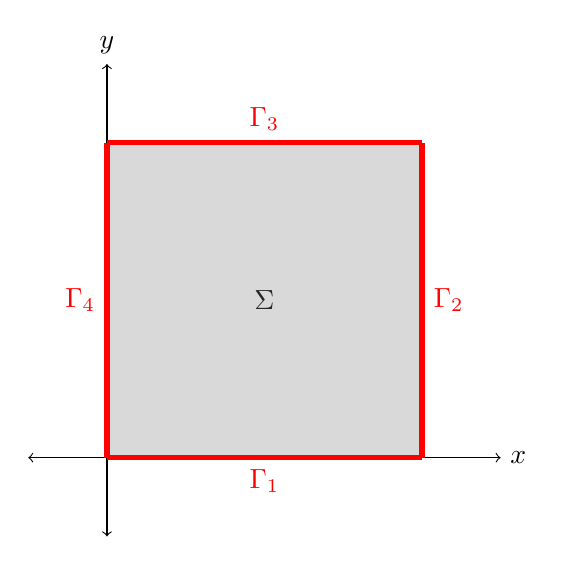
\begin{tikzpicture}
        \draw node at (2,2){$\Sigma$};
        \draw[fill=black!50, opacity=.3] (0,0) -- (4,0) -- (4,4) -- (0,4) -- cycle;
        \draw[<->] (-1,0)--(5,0) node[right]{$x$};
        \draw[<->] (0,-1)--(0,5) node[above]{$y$};
        \draw[line width=2pt,red](0,0)--(4,0) node[anchor=north] at (2,0){$\Gamma_1$};
        \draw[line width=2pt,red](4,0)--(4,4) node[anchor=west] at (4,2){$\Gamma_2$};
        \draw[line width=2pt,red](4,4)--(0,4) node[anchor=south] at (2,4){$\Gamma_3$};
        \draw[line width=2pt,red](0,4)--(0,0) node[anchor=east] at (0,2){$\Gamma_4$};
        \end{tikzpicture}
        \end{center}
    
    Then $d\Sigma = dx\wedge dy$, $d\Gamma_1 = d\Gamma_3 = dx$, and $d\Gamma_2 = d\Gamma_4 = dy$. Then let $\mathbf{F}(x,y,z)=(F_1(x,y,z),F_2(x,y,z),F_3(x,y,z))$ be an arbitrary vector field. The claim is that
    \begin{align*}
        \int_\Sigma d\flat_1(\mathbf{F}) &= \int_\Gamma \flat_1(\mathbf{F})\\
        \iff \int_\Sigma \curl \mathbf{F}\cdot \mathbf{\hat{n}}d\Sigma &= \int_\Gamma F\cdot \mathbf{t} d\Gamma.
    \end{align*}
    To see this identification fully, note $\mathbf{\hat{n}}=e_3$, $\mathbf{\hat{t}}_1=e_1$, $\mathbf{\hat{t}}_2=e_2$, $\mathbf{\hat{t}}_3=-e_1$, and $\mathbf{\hat{t}}_4=-e_2$. Then try to realize
    \[
    d\flat_1(\mathbf{F})=(\nabla \times \mathbf{F})\cdot \mathbf{\hat{n}}d\Sigma \quad \textrm{and} \quad \flat_1(\mathbf{F})=\mathbf{F}\cdot \mathbf{\hat{t}}d\Gamma.
    \]
\end{ex}

\begin{ex}{Divergence Theorem}{div_theorem}
    Draw a similar example letting 
    \[
    V = \{(x,y,z)~\vert~ 0\leq x,y,z\leq 1\}.
    \]
    Work through defining $\partial V$ and the necessary forms and fields in the same way as the previous example. 
\end{ex}











\end{document}
